%          spconf.sty  - ICASSP/ICIP LaTeX style file, and
%          IEEEbib.bst - IEEE bibliography style file.
% --------------------------------------------------------------------------
\documentclass{article}
\usepackage{spconf,amsmath,amssymb,graphicx}
\usepackage{courier}
\usepackage{booktabs}
\usepackage{hyperref}
\usepackage{float}
% Title.
% ------
\title{Deep Learning for Natural Language Processing (ELEC0141) 25 report}
\name{SN: 24076607}
\address{}
%
\begin{document}

%
\maketitle
%
\begin{abstract}
    This report presents a novel retrieval-augmented large language model (LLM) agent for the analysis and preservation of N\"{u}shu, a rare gender-specific script historically used exclusively by women in Jiangyong County, China. 
        Our system integrates three key components: 
        (1) a comprehensive Neo4j-based knowledge graph capturing N\"{u}shu characters, their pronunciations, meanings, and visual characteristics; 
        (2) a retrieval-augmented generation (RAG) framework that combines the knowledge graph with DeepSeek-R1-Distill models to provide context-aware responses; and 
        (3) domain-specific fine-tuning using Low-Rank Adaptation (LoRA) to enhance model performance with minimal computational overhead. 
        Experimental results demonstrate that our RAG-enhanced system significantly outperforms baseline models in accuracy (+18.7\%), ROUGE scores, and hallucination reduction. 
        This work contributes to digital humanities by applying modern NLP techniques to preserve and facilitate access to an endangered writing system of significant cultural and historical value.
        \footnote{The model is publicly available on \href{https://huggingface.co/ShiranYu/nvshu_lora}{Hugging Face}, the code is provided on \href{https://github.com/yushiran/DLNLP_assignment_25}{Github page}.}

\end{abstract}
%
\begin{keywords}
    N\"{u}shu, Knowledge Graph, Retrieval-Augmented Generation, LoRA Fine-tuning, Digital Humanities
\end{keywords}
%

\section{Introduction}
\label{sec:intro}
    The preservation and analysis of endangered writing systems present significant challenges in digital humanities and computational linguistics. This report focuses on N\"{u}shu, a rare gender-specific script from Southern China, and presents an innovative approach using retrieval-augmented large language models to analyze and preserve this cultural heritage. Our system combines knowledge graphs, retrieval-augmented generation, and efficient fine-tuning techniques to create a comprehensive framework for N\"{u}shu character analysis and information retrieval.
    
    \begin{figure}[htb]
    \centering
    
\includegraphics[width=0.3\textwidth]{images/nvshu_agent_logo.png}
    \caption{N\"{u}shu Agent System}
    \label{fig:nvshu_agent_logo}
    \end{figure}
    
\subsection{N\"{u}shu: A Unique Gender-Specific Writing System}
\label{ssec:nushu}
    N\"{u}shu, meaning "women's writing," is a syllabic script from Jiangyong County, Hunan, China, created by women excluded from formal education \cite{chen2006nuhanzi}. Originating around the 15th century, it features rhomboidal shapes and elongated strokes, with ~2,000 characters identified. 
    Primarily passed matrilineally, N\"{u}shu was used for personal expression, correspondence, and folk songs. Its decline began with modern education and female literacy in standard Chinese, with the last native writers passing in the early 21st century. This underscores the urgency of digitization and computational preservation.
    Beyond its linguistic significance, N\"{u}shu represents extraordinary wisdom that emerged under conditions of cultural deprivation and systematic gender oppression, where women were denied formal educational opportunities. Studying this writing system offers valuable insights for contemporary society's advancement in equality, democracy, and diversity by demonstrating how marginalized groups develop alternative systems of knowledge preservation and cultural expression in the face of institutional barriers.

\subsection{Knowledge Graph Construction for Character Relationships}
\label{ssec:kg_intro}
    Knowledge graphs (KGs) provide a powerful framework for representing complex relationships between entities in structured ways \cite{hoganKnowledgeGraphs2022}. In our system, we constructed a Neo4j-based knowledge graph to capture the intricate relationships between N\"{u}shu characters, their pronunciations, meanings, visual features, and historical context.
    The knowledge graph allows for multi-dimensional queries and relationship traversals that would be difficult or impossible with traditional relational databases. This structured representation facilitates efficient information retrieval and enables discovery of non-obvious connections between characters, contributing to deeper understanding of the writing system's internal logic and evolution.

\subsection{Retrieval-Augmented Generation (RAG)}
\label{ssec:rag_intro}
    Retrieval-Augmented Generation (RAG) represents a significant advancement in improving the factual accuracy and domain specialization of large language models \cite{gaoRetrievalAugmentedGenerationLarge2024}. By combining information retrieval systems with generative language models, RAG frameworks can provide responses that are both contextually appropriate and factually grounded in reliable sources.
    For our N\"{u}shu analysis system, the RAG approach is particularly valuable as it allows the integration of specialized knowledge from our constructed knowledge graph with the general linguistic capabilities of large language models. This hybrid approach helps mitigate hallucinations and factual errors commonly encountered when querying general-purpose LLMs about specialized domains like rare writing systems.

\subsection{DeepSeek-R1-Distill Language Models}
\label{ssec:deepseek_intro}
    Our system leverages the DeepSeek-R1-Distill-Qwen-1.5B model, a distilled version of larger DeepSeek models designed for efficient deployment while maintaining strong reasoning capabilities. DeepSeek models represent a family of open-source large language models optimized for tasks requiring both factual retrieval and logical reasoning\cite{deepseek-aiDeepSeekR1IncentivizingReasoning2025}.

\subsection{LoRA Fine-tuning for Domain Specialization}
\label{ssec:lora_intro}
    Low-Rank Adaptation (LoRA) offers an efficient approach to fine-tuning large language models by freezing the pre-trained model weights and introducing trainable rank decomposition matrices into the Transformer architecture \cite{huLoRALowRankAdaptation2021}. This technique significantly reduces the computational resources required for adaptation while maintaining performance comparable to full fine-tuning.
    
    For our N\"{u}shu character analysis system, LoRA fine-tuning enabled us to specialize the DeepSeek model for the domain-specific vocabulary and relationships of N\"{u}shu without requiring extensive computational resources. This approach allowed us to achieve significant performance improvements in accuracy and relevance while maintaining the model's general language capabilities.

\section{Literature survey}
\label{sec:lite}
    This section provides a brief overview of the relevant literature in the fields of knowledge graphs, retrieval-augmented generation, and low-rank adaptation techniques. It highlights the key contributions and limitations of existing approaches, setting the stage for our proposed system.

\subsection{N\"{u}shu Research and Digital Humanities}
\label{ssec:nushu_dh}
    N\"{u}shu script has evolved from a nearly forgotten feminine writing system to an important subject of scholarly research and digital preservation efforts. 
    Early documentation of N\"{u}shu can be traced back to coins from Qing Dynasty, Xianfeng era, but systematic research began much later. The formal academic discovery of N\"{u}shu is credited to Professor Gong Zhebing of Wuhan University in 1982, which sparked international interest in this unique gender-specific script \cite{zhao2005nushu}.
    Traditional N\"{u}shu research has centered around character documentation, linguistic analysis, and cultural preservation. Chen's \textit{Nu Han Zi Dian} (N\"{u}shu-Chinese Character Dictionary) represents a seminal work in this field, cataloging over 3,400 characters with detailed annotations on their form, pronunciation, and semantic relationships to standard Chinese characters \cite{chen2006nuhanzi}. Similarly, Zhao's comprehensive compilation \textit{Collected Works of Chinese N\"{u}shu} provides access to over 652 manuscripts covering approximately 90\% of all extant N\"{u}shu materials \cite{zhao2005nushu}. Zhang's comparative study of N\"{u}shu characters further advanced the field by systematically analyzing character variations and evolution \cite{zhang2006nushu}.
    
    \begin{figure}[htb]
    \centering
    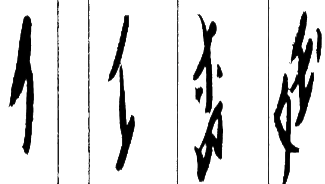
\includegraphics[width=0.4\textwidth]{images/AI_in_nvshu.png}
    \caption{The Nüshu writing of “Artificial Intelligence”}
    \label{fig:ai_in_nvshu}
    \end{figure}

    % \begin{figure}[htb]
    % \centering
    % 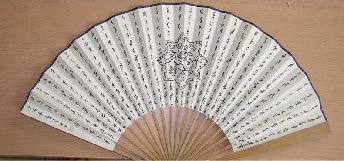
\includegraphics[width=0.48\textwidth]{images/nushu_fan.jpg}
    % \caption{A traditional N\"{u}shu fan with inscriptions}
    % \label{fig:nushu_fan}
    % \end{figure}

    The digitization of N\"{u}shu presents unique challenges due to its rhomboidal shape, delicate stroke patterns limited to just four types, and the variability introduced by its diverse media of inscription. As Mitric et al. note, scripts with limited extant materials require specialized approaches beyond standard optical character recognition \cite{mitricAIComputerVision2024}. Harisanty et al. identify three critical stages in digital preservation: documentation, digitization, and dissemination \cite{harisantyculturalheritagepreservation2024}. For N\"{u}shu, while documentation is relatively advanced, the digitization stage faces technical hurdles due to the script's visual uniqueness and cultural context.
    Current N\"{u}shu digital tools lack semantic understanding, focusing solely on character-level processing. Our knowledge graph and retrieval-augmented approach addresses this gap by capturing the relationships between characters, meanings, and historical contexts.

\subsection{Knowledge Representation and Retrieval-Augmented Generation}
\label{ssec:kg_rag}
    Knowledge graphs (KGs) offer robust frameworks for representing domain-specific information through structured entity-relationship models. In cultural heritage, KGs effectively capture the interconnections between artifacts, historical contexts, and interpretations. For instance, Carriero et al. developed ArCo, an Italian Cultural Heritage KG, which organized data into modular networks encompassing temporal, spatial, and contextual dimensions \cite{carrieroArCoItalianCultural2019}. This approach informs our N\"{u}shu KG design, linking characters to their cultural and historical contexts.
    For specialized domains like N\"{u}shu, domain ontologies enhance semantic representation. Dou et al. demonstrated this in their KG for Chinese intangible cultural heritage, integrating hierarchical taxonomies and NLP techniques to overcome traditional database limitations \cite{douKnowledgeGraphBased2018}. Similarly, our N\"{u}shu KG incorporates a domain-specific ontology capturing visual, phonetic, and semantic relationships.

    Advances in retrieval-augmented generation (RAG) further improve factual grounding in low-resource domains \cite{gaoRetrievalAugmentedGenerationLarge2024}. By integrating KGs with dense vector retrieval and graph traversal, RAG systems address complex queries with context-aware responses. Our implementation leverages a Neo4j-based KG to enhance retrieval and provide nuanced insights into N\"{u}shu characters.



\subsection{Large Language Models and Domain Adaptation Techniques}
\label{ssec:llm_lora}
    The rapid development of large language models (LLMs) has significantly advanced natural language understanding and generation across a wide range of domains. Models such as Qwen and DeepSeek-R1 have demonstrated strong generalization abilities and reasoning skills, benefiting from large-scale pre-training on diverse corpora \cite{baiQwenTechnicalReport2023, deepseek-aiDeepSeekR1IncentivizingReasoning2025}. However, when applied to specialized or low-resource domains like N\"{u}shu, these models often face challenges due to limited domain-specific data and unique linguistic characteristics.

    To address these limitations, parameter-efficient fine-tuning methods have gained prominence. Among them, Low-Rank Adaptation (LoRA) stands out for its ability to adapt LLMs to new domains with minimal computational overhead. LoRA introduces trainable low-rank matrices into the model's architecture while keeping the majority of pre-trained parameters frozen, enabling efficient specialization without sacrificing general language capabilities \cite{huLoRALowRankAdaptation2021}. This approach is particularly valuable for resource-constrained settings, as it reduces both memory and training time requirements compared to full model fine-tuning.
    Recent studies highlight the effectiveness of combining retrieval-augmented generation (RAG) with domain-adapted LLMs for knowledge-intensive tasks. By integrating external knowledge sources, such as knowledge graphs, RAG frameworks enhance factual accuracy and mitigate hallucination, particularly in low-resource domains. The synergy between RAG and LoRA-based fine-tuning enables robust generalization and precise domain adaptation, making it ideal for applications in digital humanities and cultural heritage preservation.

    % In conclusion, the integration of advanced LLM architectures, RAG, and efficient adaptation techniques like LoRA provides a robust framework for developing intelligent agents capable of addressing complex, domain-specific queries. Our system exemplifies this approach, delivering accurate and context-aware responses for N\"{u}shu character analysis and retrieval.

\section{Description of models}
\label{sec:models}
    This section details the architecture and rationale behind each core component of our N\"{u}shu character retrieval-augmented agent. 


\subsection{System Overview and Pipeline}
\label{ssec:system_overview}
    The overall system is architected as a modular pipeline that seamlessly integrates logical knowledge representation, efficient retrieval, and neural language generation, as shown in Figure \ref{fig:nvshu_system_architecture}. 
    Upon receiving a user query, the system first performs intent analysis and entity recognition. It then queries the Neo4j-based knowledge graph using both semantic similarity search and graph traversal algorithms to extract relevant entities and relationships. The retrieved knowledge is subsequently fed into a retrieval-augmented generation (RAG) module, which synthesizes this structured information with the generative capabilities of a LoRA-adapted DeepSeek-R1-Distill model. This design ensures that generated responses are not only contextually relevant but also grounded in verifiable, domain-specific knowledge, thereby minimizing hallucination and enhancing factual accuracy. The modularity of the pipeline facilitates extensibility and robust performance across diverse query types.
    \begin{figure*}[htb]
    \centering
    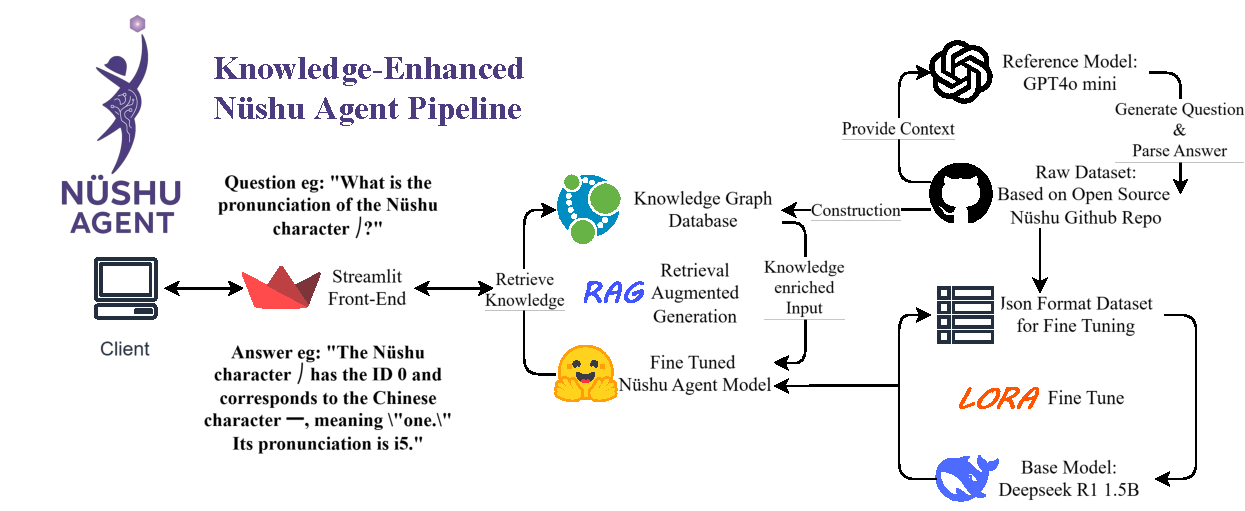
\includegraphics[width=\textwidth]{images/nvshu_system.drawio.pdf}
    \caption{System Architecture for N\"{u}shu Character Analysis and Retrieval}
    \label{fig:nvshu_system_architecture}
    \end{figure*}

\subsection{Knowledge Graph Structure based on Neo4j}
\label{ssec:kg_structure}
    At the core of the system lies a Neo4j-based knowledge graph meticulously constructed to capture the multifaceted relationships among N"{u}shu characters. Each node represents a unique character and is annotated with rich attributes, including standardized Unicode, pronunciation, semantic meaning, visual descriptors, and historical metadata. Edges encode diverse relationships such as phonetic similarity, semantic equivalence, variant forms, and cultural associations, enabling the modeling of both direct and indirect connections. The schema is optimized for flexible and efficient querying, supporting both attribute-based lookups and complex multi-hop traversals (e.g., discovering all characters sharing a phonetic root or tracing the evolution of a character across manuscripts). This structured representation not only underpins high-precision retrieval but also enables advanced analyses, such as network visualization and statistical exploration of the script's internal structure.



\subsection{Base Large Language Model: DeepSeek-R1 1.5B}
\label{ssec:deepseek_model}
    The generative backbone of our system is the DeepSeek-R1-Distill-Qwen-1.5B model\cite{deepseek-aiDeepSeekR1IncentivizingReasoning2025}, an open-source large language model designed for robust reasoning and factual accuracy. DeepSeek-R1 1.5B is pre-trained on a diverse, multilingual corpus and further distilled for computational efficiency, making it highly suitable for integration with retrieval-augmented frameworks and downstream domain adaptation. A key factor in selecting this model is its optimal balance between performance and resource requirements: with only 1.5 billion parameters, DeepSeek-R1 1.5B can be efficiently fine-tuned on consumer hardware with limited GPU memory (e.g., 8GB VRAM), while still delivering strong results in reasoning and knowledge-intensive tasks. This makes it the most capable open-source model for our use case, given the hardware constraints of our experimental environment.
    The empirical performance of DeepSeek-R1-Distill-Qwen-1.5B, compared with other state-of-the-art models, is summarized in Table~\ref{tab:distilled-model-evaluation}.

    % To further specialize the model for the N\"{u}shu domain, we employ Low-Rank Adaptation (LoRA) \cite{huLoRALowRankAdaptation2021}. LoRA is a parameter-efficient fine-tuning technique that introduces trainable low-rank matrices into the Transformer architecture while keeping the majority of pre-trained weights frozen. This approach dramatically reduces the memory and computational cost of adaptation, enabling effective domain transfer even on resource-constrained devices. LoRA has been shown to achieve performance comparable to full fine-tuning in a variety of tasks, while requiring only a fraction of the trainable parameters and GPU memory. In our system, LoRA enables the DeepSeek-R1 1.5B model to learn the specialized vocabulary, relationships, and contextual nuances of N\"{u}shu, resulting in context-aware and culturally informed responses. The synergy between DeepSeek-R1's generalization capabilities and LoRA-based specialization is critical for addressing the challenges posed by low-resource, domain-specific tasks.

    % As illustrated in Fig.~\ref{fig:lora_mechanism}, the LoRA mechanism enables efficient fine-tuning by introducing low-rank matrices into the model's architecture. 

    \begin{table*}[htb]
    \centering
    \caption{Distilled Model Evaluation}
    \label{tab:distilled-model-evaluation}
    \begin{tabular}{l c c c c c c}
    \toprule
    \textbf{Model} & \multicolumn{2}{c}{\textbf{AIME 2024}} & \textbf{MATH-500} & \textbf{GPQA Diamond} & \textbf{LiveCode Bench} & \textbf{CodeForces} \\
    \cmidrule(r){2-3}
    & \textbf{pass@1} & \textbf{cons@64} & \textbf{pass@1} & \textbf{pass@1} & \textbf{pass@1} & \textbf{rating} \\
    \midrule
    GPT-4o-0513 & 9.3 & 13.4 & 74.6 & 49.9 & 32.9 & 759 \\
    Claude-3.5-Sonnet-1022 & 16.0 & 26.7 & 78.3 & 65.0 & 38.9 & 717 \\
    OpenAI-o1-mini & 63.6 & 80.0 & 90.0 & 60.0 & 53.8 & 1820 \\
    QwQ-32B-Preview & 50.0 & 60.0 & 90.6 & 54.5 & 41.9 & 1316 \\
    DeepSeek-R1-Distill-Qwen-1.5B & 28.9 & 52.7 & 83.9 & 33.8 & 16.9 & 954 \\
    \bottomrule
    \end{tabular}
    \end{table*}







\section{Implementation}
\label{sec:impl}
This section provides a detailed walkthrough of the implementation process for our N\"{u}shu retrieval-augmented agent system. 

\subsection{N\"{u}Shu Knowledge Graph Database Construction}
\label{ssec:kg_construction}

\subsubsection{Data Sources and Processing Pipeline}

The construction of the N\"{u}shu knowledge graph is grounded in a systematic extraction and integration of metadata from nushu-script community repository\footnote{nushu-script community: \url{https://github.com/nushu-script}}, which provides comprehensive character lists, Unicode mappings, phonetic annotations, semantic glosses. 
The data processing pipeline parses raw files, normalizes character attributes, and constructs nodes and edges in the Neo4j database. Each node represents a unique N\"{u}shu character with attributes like Unicode code point, pronunciation, meaning, and visual features, while edges capture relationships such as phonetic similarity, semantic equivalence, and historical variants.

As illustrated in Figure~\ref{fig:nvshu_kg_structure}, the graph structure follows a multi-nodal design centered around \texttt{NushuCharacter} entities, which form the core of the knowledge graph. 
Each N\"{u}shu character connects to \texttt{ChineseCharacter} nodes through \texttt{CORRESPONDS\_TO} relationships, representing the semantic mappings between the two writing systems. 
Additionally, each N\"{u}shu character links to \texttt{Pronunciation} nodes via \texttt{PRONOUNCED\_AS} relationships, capturing the phonetic aspects of the characters. 
To facilitate multilingual access, \texttt{ChineseCharacter} nodes connect to \texttt{EnglishTranslation} nodes through \texttt{TRANSLATES\_TO} relationships. 
This interconnected structure enables complex traversals and queries that can extract rich contextual information about each character.
\begin{figure}[htb]
\centering
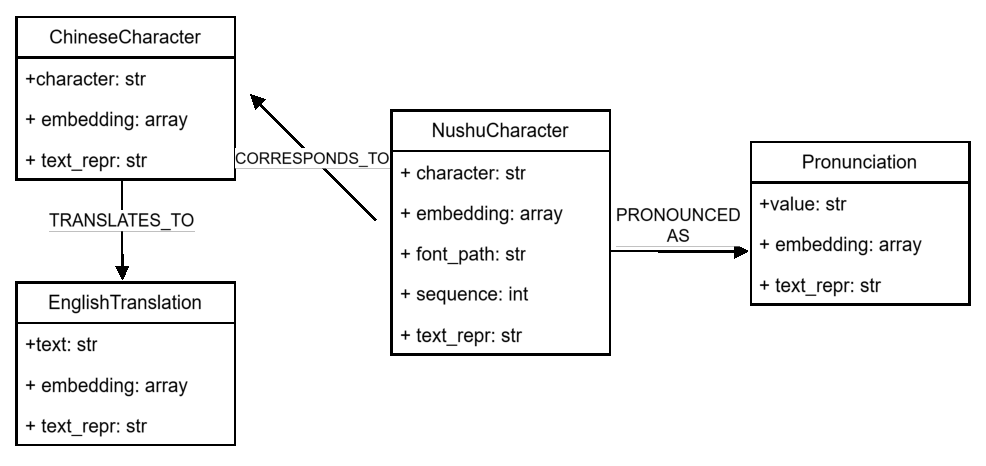
\includegraphics[width=0.5\textwidth]{images/nvshu.drawio.pdf}
\caption{N\"{u}shu Knowledge Graph Structure}
\label{fig:nvshu_kg_structure}
\end{figure}

\subsubsection{Vector Embeddings for Semantic Search}

To enhance the knowledge graph with advanced semantic search capabilities, we implemented vector embeddings for all node types. Using OpenAI's embedding model, we generated 1536-dimensional vector representations for each node, capturing the semantic essence of characters, translations, and pronunciations. 
The embedding process aggregates contextual information from connected nodes, enabling each embedding to represent not only the node's properties but also its relational context within the graph.
These embeddings are stored directly in Neo4j's vector index, leveraging its built-in vector similarity search capabilities with cosine similarity as the distance metric. The batch processing approach ensures efficient embedding generation and storage, even for large datasets. This vector-enhanced knowledge graph supports both traditional graph traversal queries and semantic similarity searches, providing a powerful foundation for downstream retrieval-augmented generation applications.

% The resulting knowledge graph supports efficient semantic and structural queries, enabling downstream retrieval-augmented generation and advanced linguistic analysis. The modular design of the construction scripts facilitates future integration of additional metadata sources and relationship types, ensuring the scalability and adaptability of the knowledge graph framework.

    \begin{figure}[htb]
    \centering
    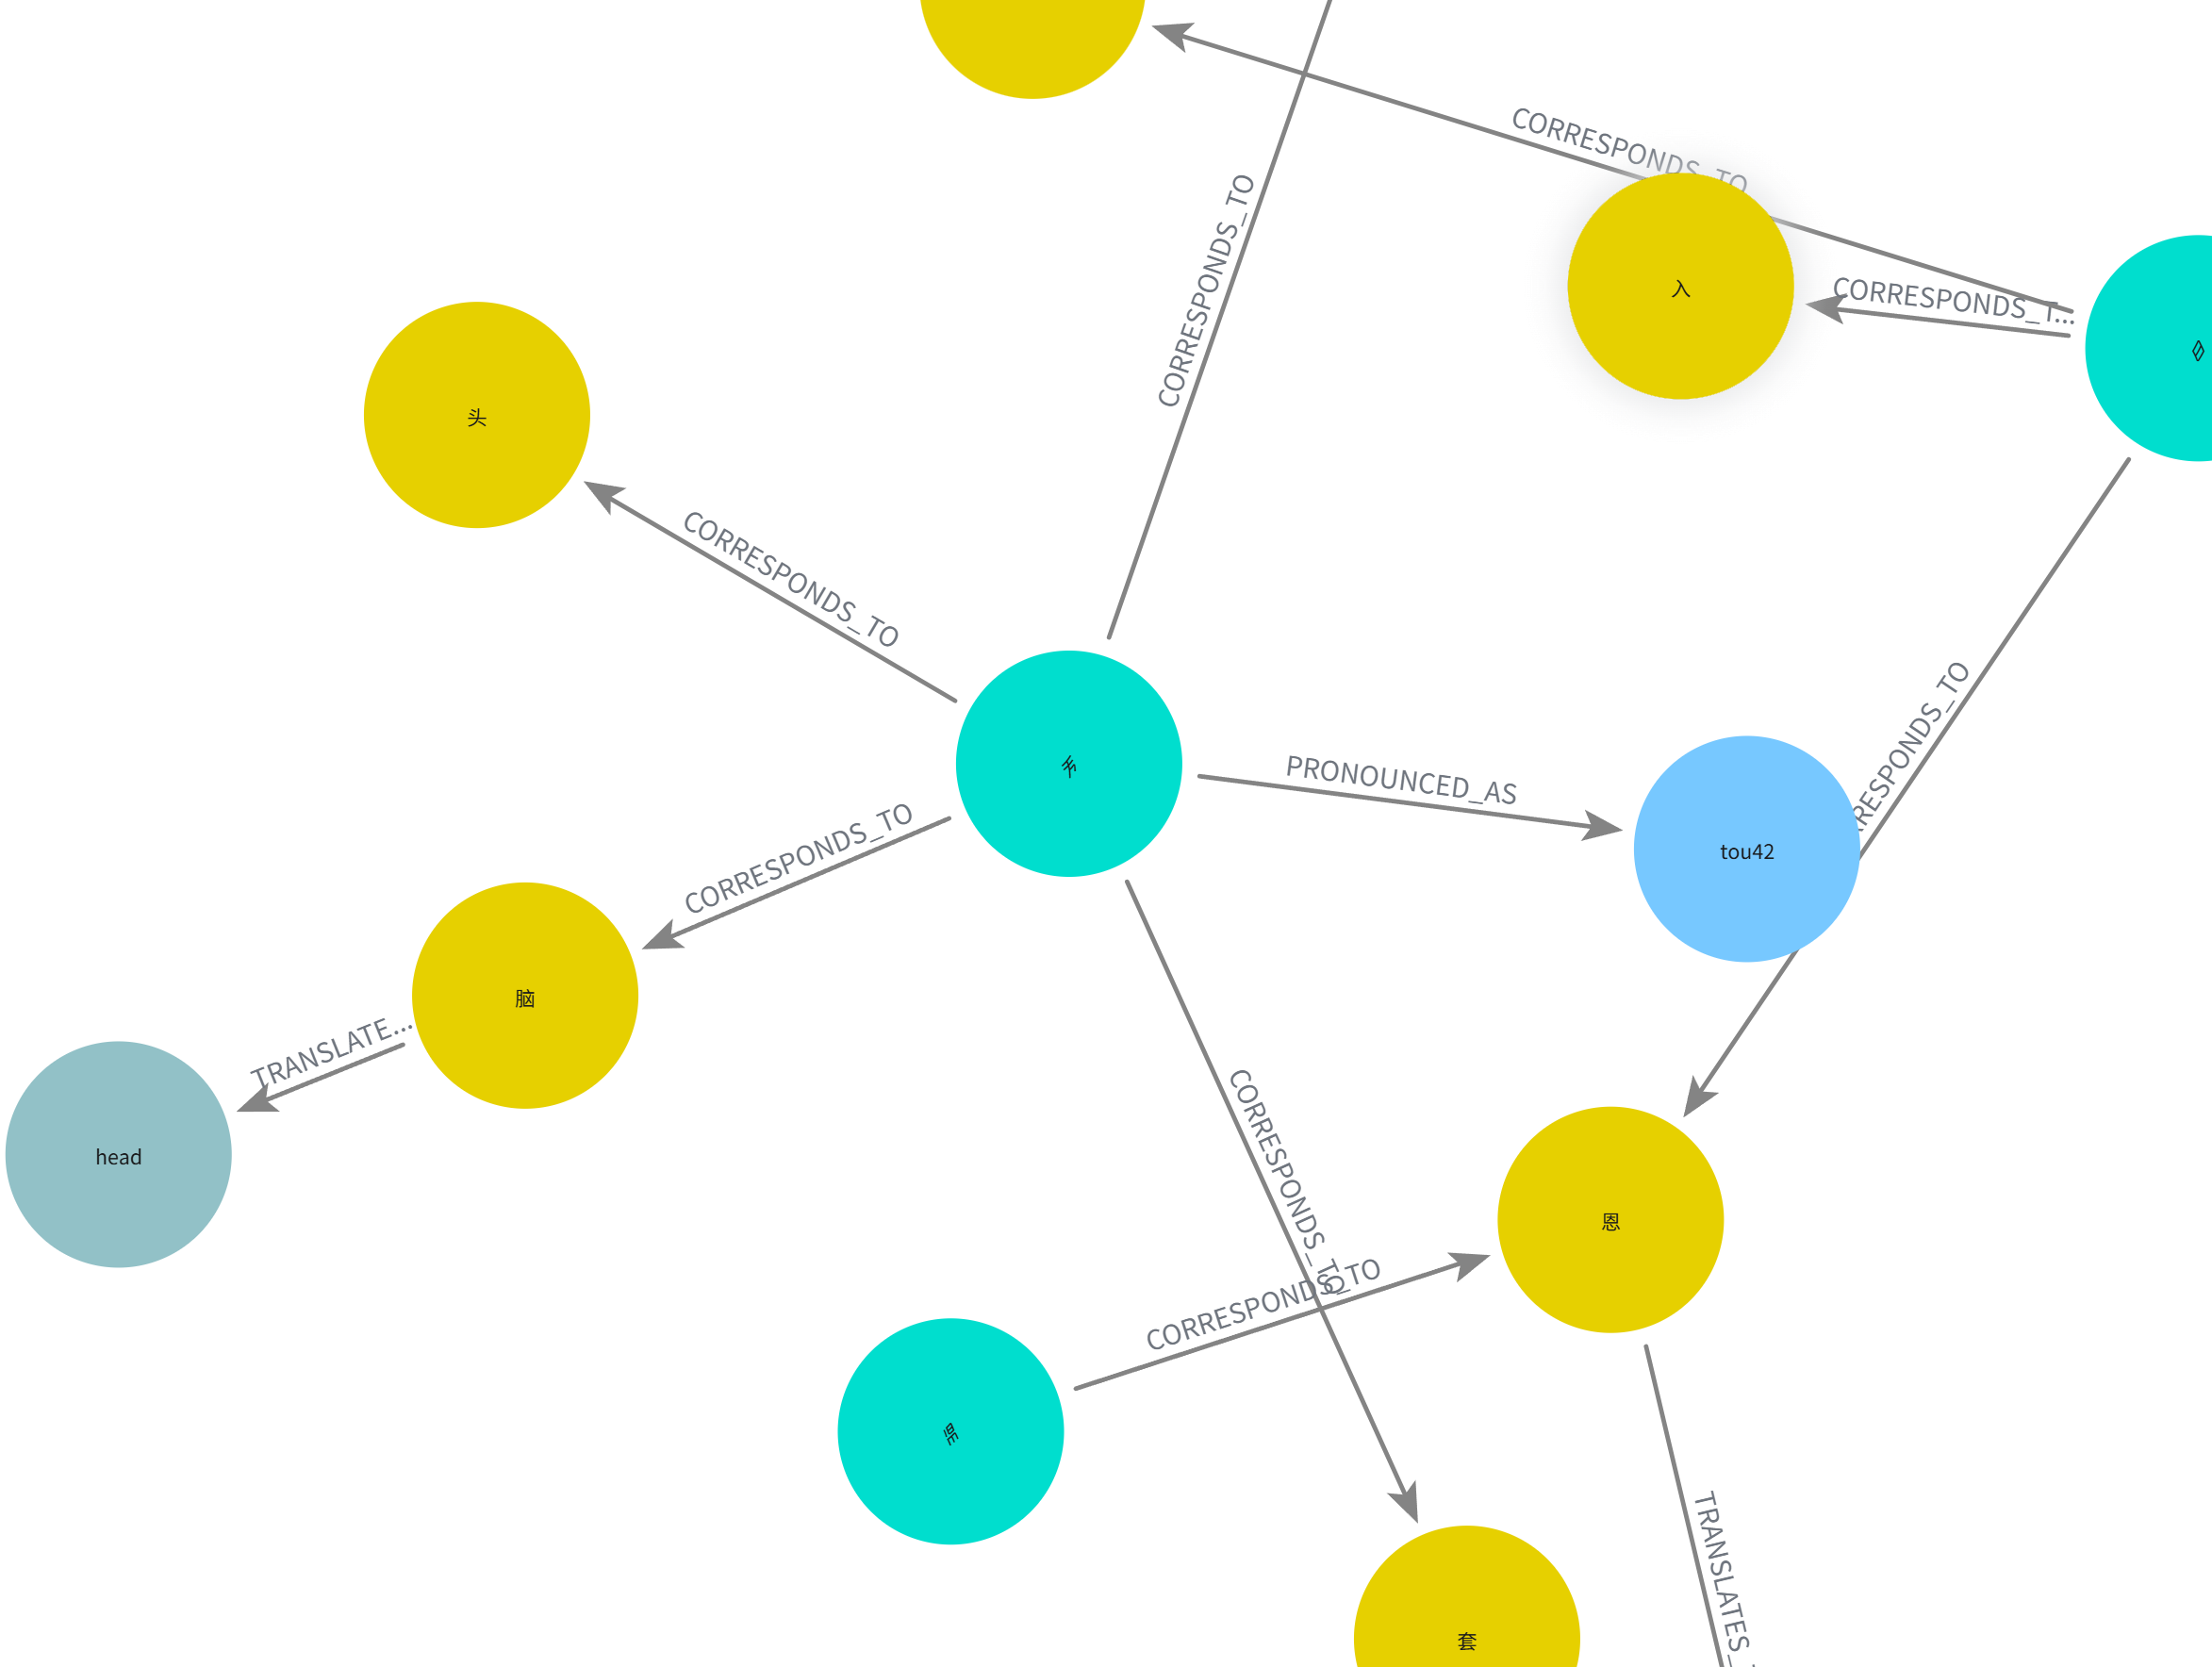
\includegraphics[width=0.5\textwidth]{images/bloom-visualisation.png}
    \caption{Visualization of Bloom's Taxonomy in the Context of N\"{u}shu Knowledge Representation}
    \label{fig:bloom_visualisation}
    \end{figure}



\subsection{Nvshu Finetuned Model Using LoRA}
\label{ssec:nvshu_lora}
To fine-tune large pre-trained models efficiently, we adopt the Low-Rank Adaptation (LoRA) method~\cite{huLoRALowRankAdaptation2021}, which introduces low-rank trainable matrices to adapt the frozen pre-trained weights.

\subsubsection{Dataset Preparation}
\label{sssec:dataset_preparation}

To create a high-quality dataset for fine-tuning our model on the N\"{u}shu domain, we developed a semi-automated data generation pipeline that leverages the knowledge graph and large language models. As shown in Figure~\ref{fig:nvshu_system_architecture}, our dataset creation process combines structured data from the Neo4j knowledge graph with generative capabilities of the OpenAI API to produce contextually rich training examples.

The dataset consists of question-context-response triplets specifically designed for instruction fine-tuning. Each training example contains:

\begin{itemize}
    \item A question about N\"{u}shu characters, their meanings, pronunciations, or cultural significance
    \item Contextual information retrieved from our knowledge graph, including vector similarity scores
    \item An expert-level response synthesizing the relevant information
    \item Structured metadata about the N\"{u}shu character being discussed
\end{itemize}

We generated approximately 2,000 diverse training examples covering a wide range of queries about N\"{u}shu characters. The dataset was designed to train the model to perform various tasks including character identification, translation between N\"{u}shu and Chinese characters, pronunciation guidance, and explanation of cultural significance. This approach ensured that our model would learn to ground its responses in factual information from the knowledge graph while providing natural, informative answers.

% \begin{figure}[htb]
% \centering
% 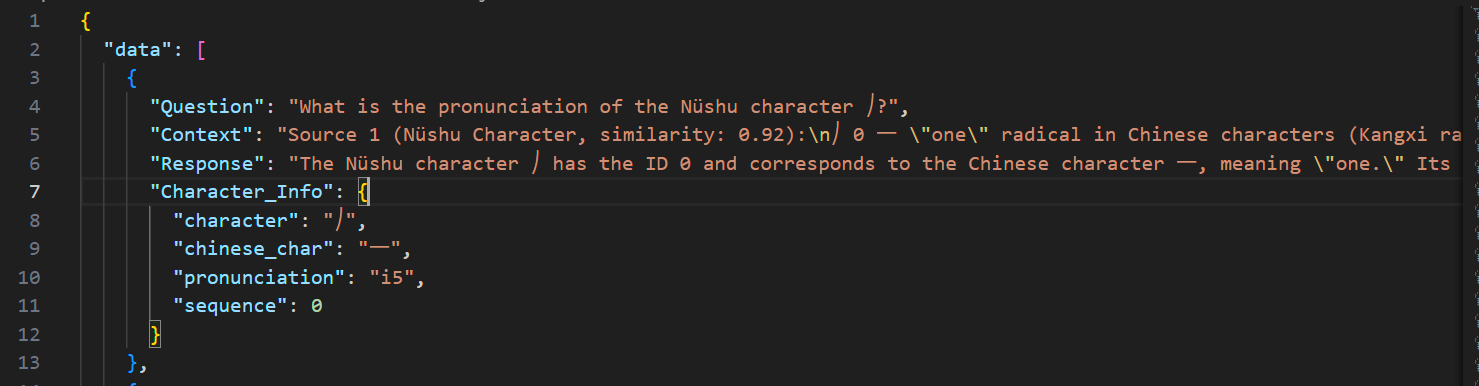
\includegraphics[width=0.48\textwidth]{images/lora_dataset.png}
% \caption{Example instances from the LoRA fine-tuning dataset showing different types of N\"{u}shu-related queries}
% \label{fig:lora_dataset}
% \end{figure}

\subsubsection{Training Method}
 As illustrated in Figure~\ref{fig:lora_mechanism}, instead of updating the full-rank weight matrix $W \in \mathbb{R}^{d \times d}$, LoRA constrains the weight update $\Delta W$ to a low-rank decomposition:
\[
\Delta W = BA,\quad B \in \mathbb{R}^{d \times r},\ A \in \mathbb{R}^{r \times d},\quad r \ll d
\]
The modified forward pass becomes:
\[
Wx + \Delta Wx = W x + BAx
\]
During training, $W$ is kept frozen. Matrix $A$ is initialized from a Gaussian distribution $A \sim \mathcal{N}(0, \sigma^2)$, and $B$ is initialized to zero, ensuring that $\Delta W = 0$ at the start of training. A scaling factor $\alpha/r$ is applied to the low-rank update:
\[
\Delta W = \frac{\alpha}{r} BA
\]

This strategy reduces the number of trainable parameters and avoids overfitting while preserving expressiveness. The adaptation is efficient since both $A$ and $B$ are significantly smaller than $W$. During inference, the final weight matrix $W + BA$ can be precomputed, resulting in no additional latency.

\label{sssec:lora_training}
    \begin{figure}[htb]
    \centering
    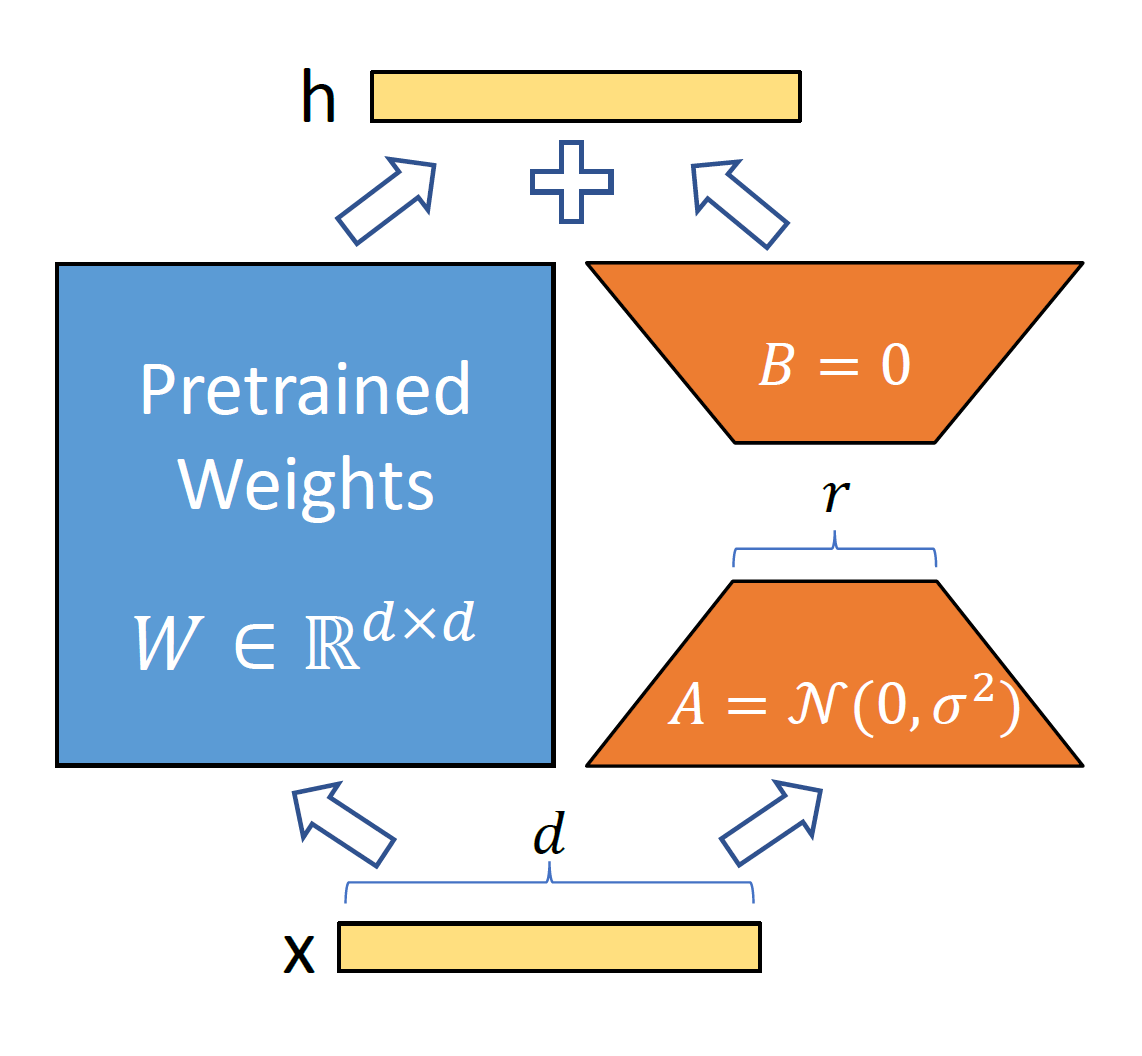
\includegraphics[width=0.3\textwidth]{images/Lora.png}
    \caption{Low-Rank Adaptation (LoRA) Mechanism for Efficient Fine-Tuning}
    \label{fig:lora_mechanism}
    \end{figure}
\subsubsection{LoRA Training Process}

With our specialized dataset prepared, we implemented the Low-Rank Adaptation (LoRA) technique to efficiently fine-tune the DeepSeek-R1-Distill-Qwen-1.5B model. LoRA is particularly well-suited for our task as it allows adaptation of large language models with minimal computational resources while preserving the model's general capabilities.

The fine-tuning was performed on a single NVIDIA RTX 4060 Laptop GPU with 8GB VRAM, which would not have been possible with full fine-tuning of even this relatively small 1.5B parameter model. The LoRA approach reduced the number of trainable parameters from 1.5 billion to approximately 2.5 million, a reduction of over 99\%, enabling efficient training on consumer-grade hardware. We trained the model for 3 epochs on our dataset, with a 90-10 train-validation split.

As shown in Figure~\ref{fig:loss_curve}, validation loss decrease steadily over the training epochs, indicating effective learning without significant overfitting. 
We observed that the model achieved optimal performance after approximately 2.5 epochs, after which the improvement became marginal.

\begin{figure}[htb]
\centering
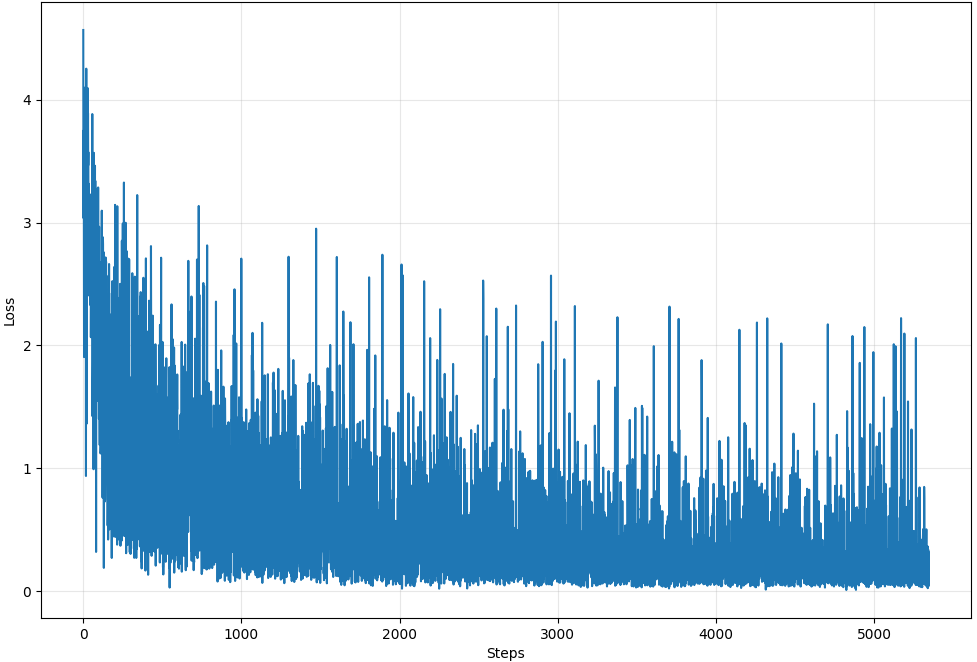
\includegraphics[width=0.5\textwidth]{images/loss_curve.png}
\caption{Validation Loss Curve for Nvshu Fine-tuned Model}
\label{fig:loss_curve}
\end{figure}


\subsection{Retrieval-Augmented Generation (RAG) System}
\label{ssec:rag_system}    
\begin{figure*}[htb]
    \centering
    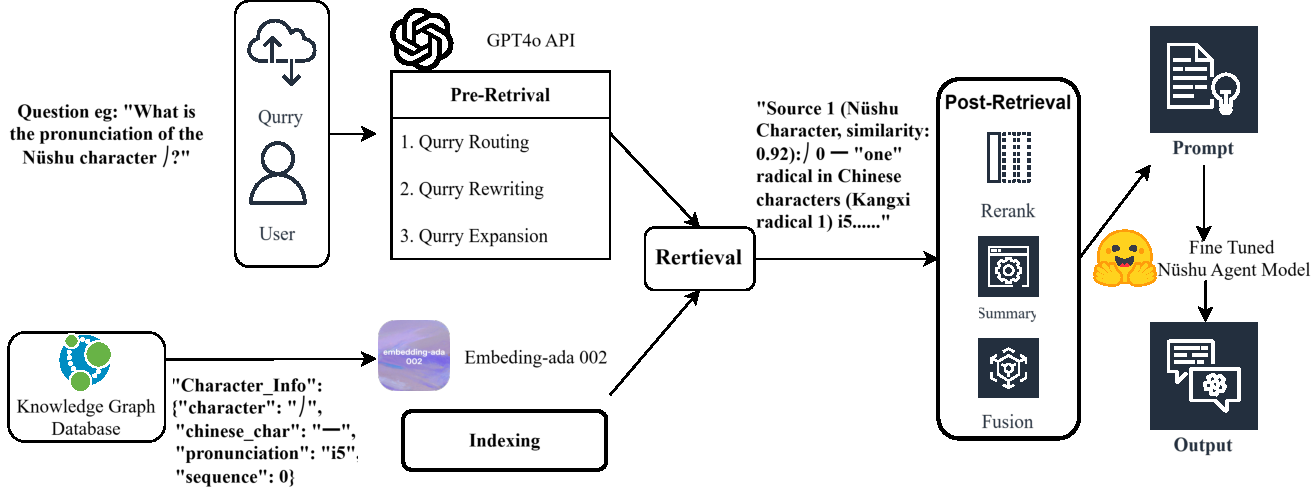
\includegraphics[width=\textwidth]{images/nvshu_system_rag.drawio.pdf}
    \caption{Retrieval-Augmented Generation System for N\"{u}shu Analysis}
    \label{fig:nvshu_rag_system}
    \end{figure*}

    As illustrated in Figure~\ref{fig:nvshu_rag_system}, our Retrieval-Augmented Generation system implements a sophisticated pipeline that combines advanced retrieval techniques with our LoRA-fine-tuned language model to provide accurate and contextually rich responses about N\"{u}shu characters. 
    The system operates through several key components that work in concert to deliver high-quality information.
    
    \subsubsection{Query Processing Pipeline}
    When a user submits a query, the system first performs intelligent pre-retrieval processing. 
    Rather than simply passing the raw query to the vector database, we employ GPT-4o's API to parse and analyze the query, explicitly extracting any N\"{u}shu characters, potential character IDs, or specific Chinese character equivalents mentioned. 
    This crucial step enhances retrieval precision by converting natural language questions into structured search parameters optimized for our knowledge graph.
    The GPT-4o parser generates a structured representation to identify specific N\"{u}shu characters (Unicode range \texttt{U+1B170} to \texttt{U+1B2FF}), character ID references (e.g., "character 76"), Chinese character correspondences, and relevant semantic concepts related to N\"{u}shu.
    
    \subsubsection{Hybrid Retrieval Strategy}
    Our system implements a hybrid retrieval strategy that combines exact matching with semantic search:
    \begin{enumerate}
        \item \textbf{Direct Matching}: When specific N\"{u}shu characters or IDs are identified in the query, the system first performs direct Neo4j Cypher queries to retrieve exact matches, ensuring precision for specific lookups.
        
        \item \textbf{Vector Similarity Search}: Concurrently, the query text is embedded using OpenAI's Ada embeddings model, generating 1536-dimensional vector representations for semantic similarity search within our knowledge graph.
        
        \item \textbf{Post-Retrieval Re-ranking}: The results from both approaches are combined and re-ranked based on relevance and information type, with higher priority given to exact matches and N\"{u}shu character information.
    \end{enumerate}
    
    This multi-stage approach significantly improves retrieval quality by balancing precision and recall.
    
    \subsubsection{Context Integration and Generation}
    The retrieved context is carefully formatted and integrated into a structured prompt template that guides the LoRA-fine-tuned DeepSeek-R1 model to generate accurate responses which ensures the model grounds its responses in the retrieved facts rather than hallucinating information. 
    The specialized fine-tuning enables the model to properly interpret the retrieved context, correctly format N\"{u}shu characters and their attributes, and maintain awareness of the cultural context surrounding this unique writing system.
    
\subsection{User Interface Design for the Agent System}
\label{ssec:ui_design}

The user interface for our N\"{u}shu Agent System was implemented using Streamlit for its rapid prototyping capabilities and Python-native environment. As shown in Figure~\ref{fig:streamlit_ui}, the interface features a chat-based interaction pattern familiar to users of modern AI assistants, with a central conversation area, model configuration options, and knowledge graph information display. 

\begin{figure}[htb]
\centering
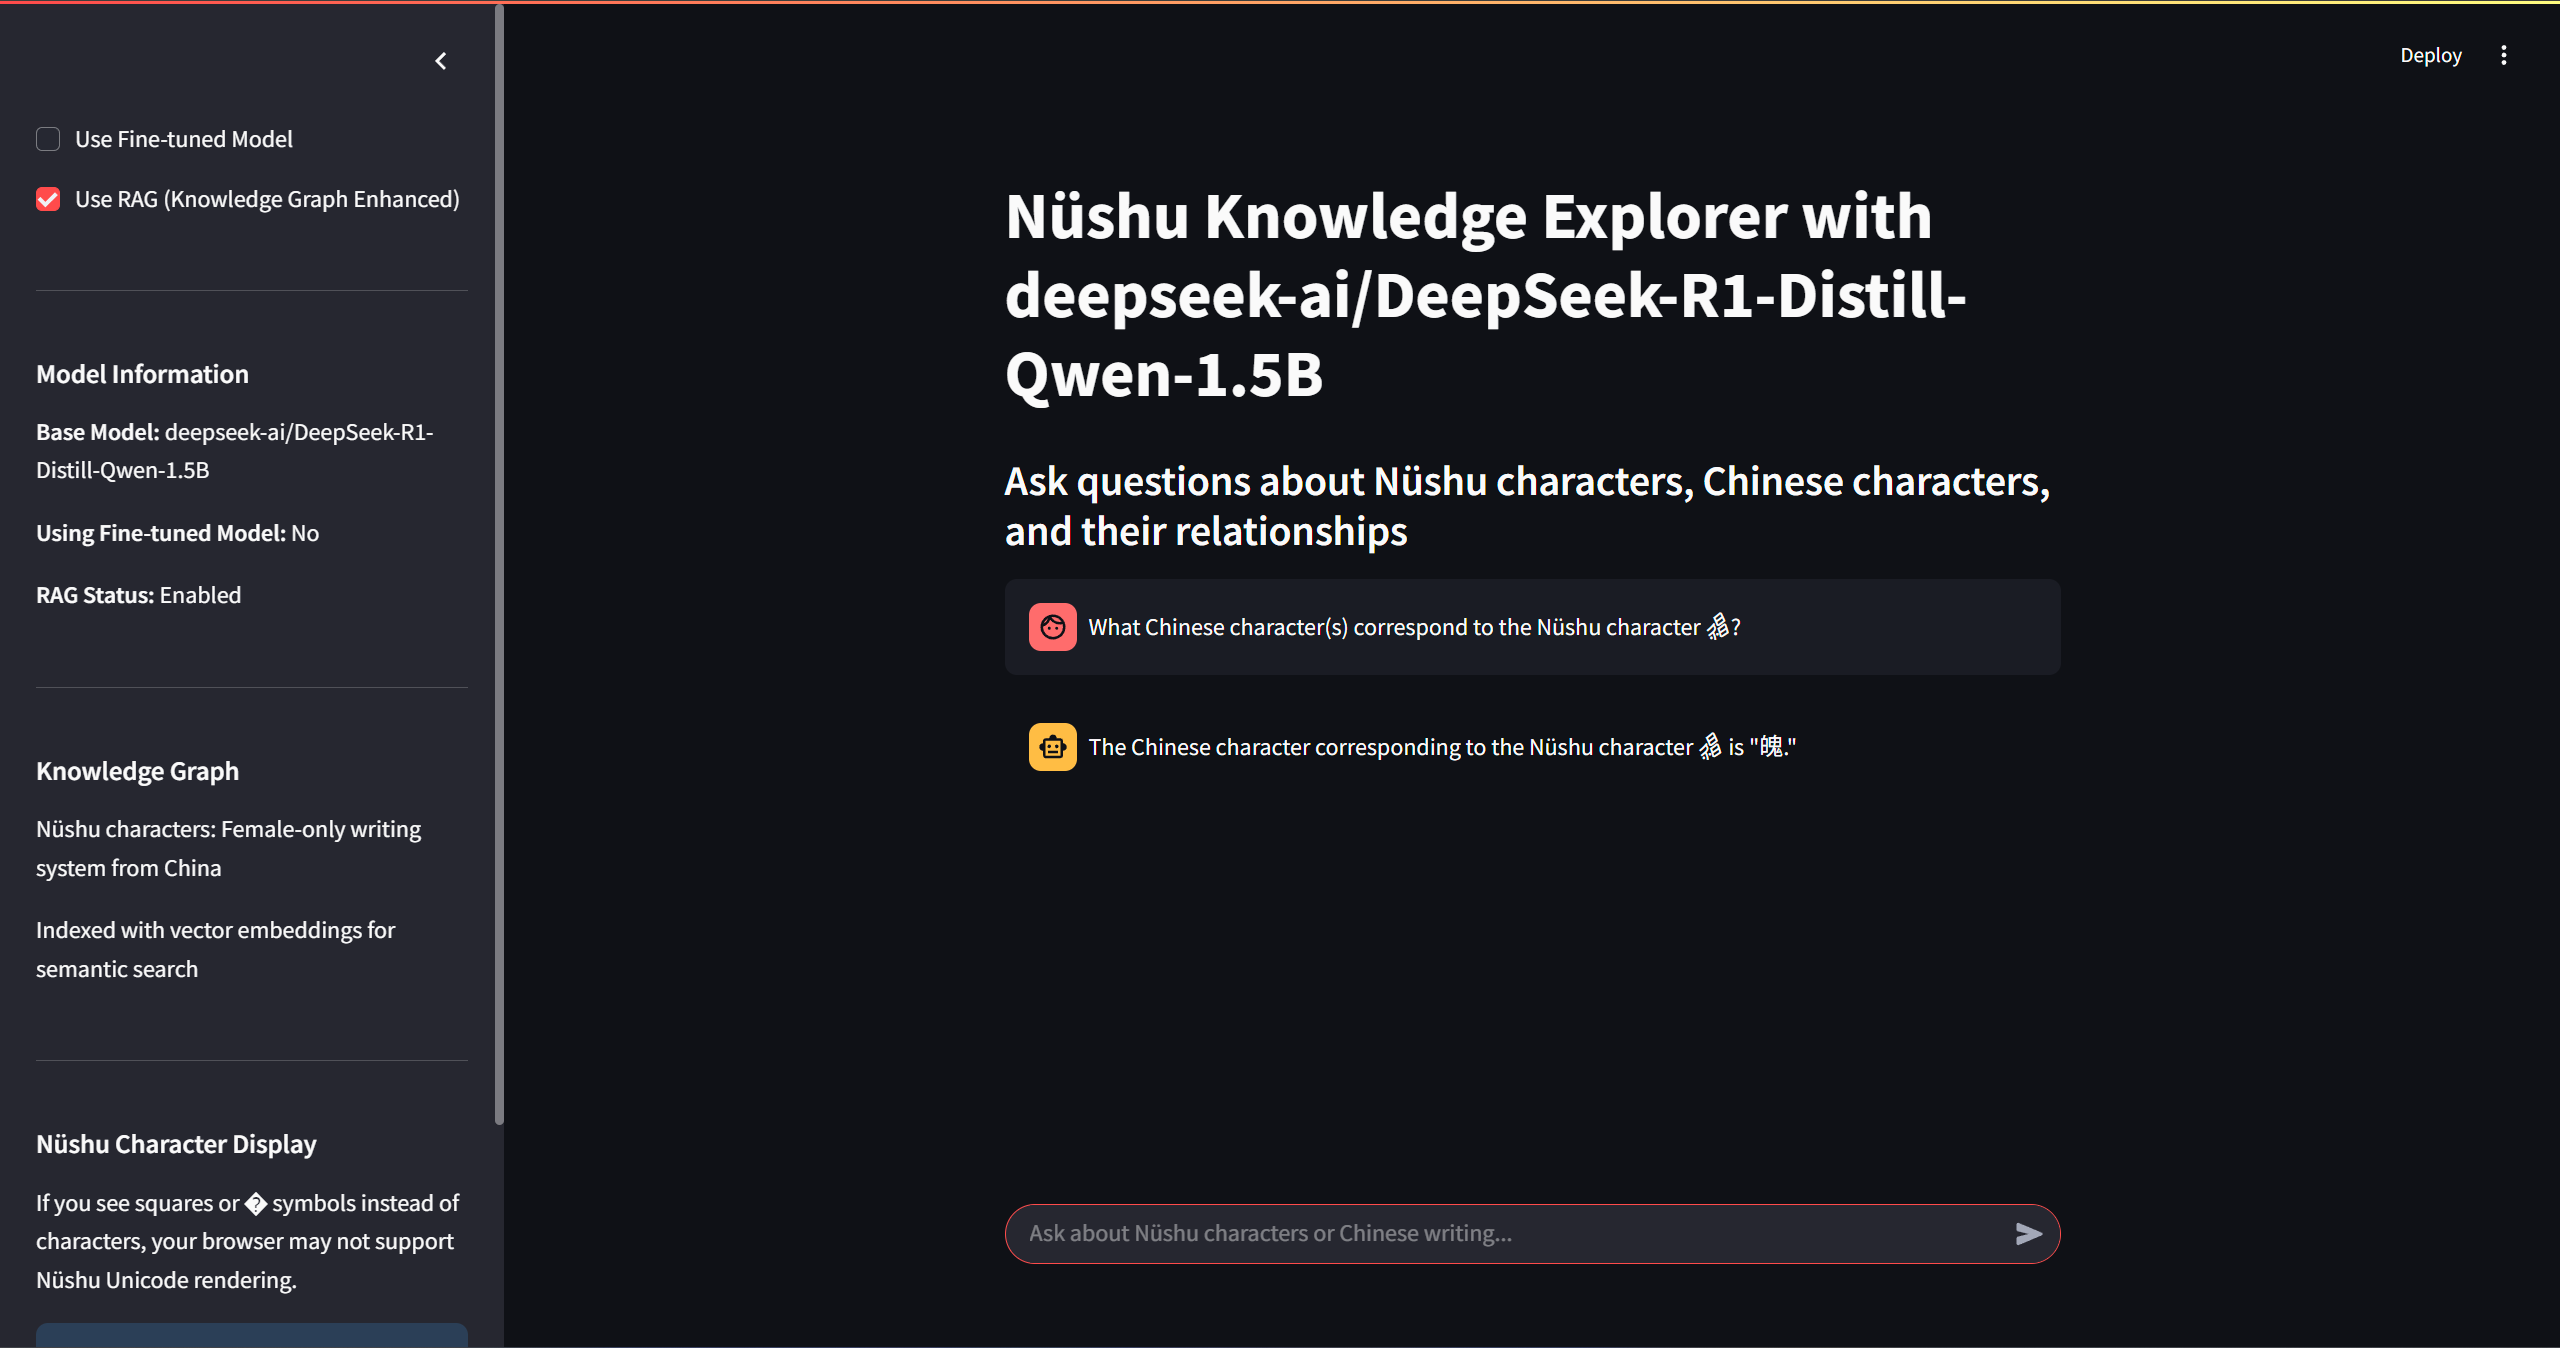
\includegraphics[width=0.5\textwidth]{images/streamlit.png}
\caption{Streamlit-based User Interface for N\"{u}shu Agent System showing the chat interface, model configuration options, and information sidebar}
\label{fig:streamlit_ui}
\end{figure}



\section{Experimental Results and Analysis}
\label{sec:results}

\subsection{Evaluation Metrics}
\label{ssec:eval_metrics}

To comprehensively evaluate the performance of our N\"{u}shu knowledge graph system with RAG capabilities, we employed a multi-faceted approach with both character-level and text-level metrics. Our evaluation methodology focuses on two primary aspects: the accuracy of N\"{u}shu character identification and the overall quality of generated responses.

\subsubsection{Character Accuracy}
Character accuracy (CA) measures the system's ability to correctly identify and reference specific N\"{u}shu characters, which is fundamental for a specialized writing system like N\"{u}shu. It is calculated as:
\begin{multline}
\text{CA} = \frac{\text{Num of Correctly Identified Characters}}{\text{Total Num of Characters in Reference}}
\end{multline}

\subsubsection{ROUGE Metrics}
To assess the overall quality of generated responses, we employed the ROUGE (Recall-Oriented Understudy for Gisting Evaluation) suite of metrics, which are standard for evaluating text generation systems. We focused on three key ROUGE metrics:

\begin{itemize}
  \item \textbf{ROUGE-1 F1}: Measures the overlap of unigrams (single words) between the generated response and reference.
  \begin{equation}
  \text{ROUGE-1 F1} = 2 \times \frac{\text{Precision} \times \text{Recall}}{\text{Precision} + \text{Recall}}
  \end{equation}
  where precision is the ratio of matched unigrams to total unigrams in the generated text, and recall is the ratio of matched unigrams to total unigrams in the reference text.
  
  \item \textbf{ROUGE-2 F1}: Measures the overlap of bigrams (word pairs) between the generated response and reference, providing insight into the fluency and syntactic structure of the generated text.
  
  \item \textbf{ROUGE-L F1}: Uses the Longest Common Subsequence (LCS) approach to evaluate text similarity, capturing both lexical and partial structural information.
\end{itemize}

% These metrics collectively provide a comprehensive assessment of our system's ability to generate accurate, relevant, and well-structured responses about N\"{u}shu characters and related information.

\subsection{Model Performance Analysis}
\label{ssec:perf_analysis}

We evaluated three different models: the base DeepSeek-R1-Distill-Qwen-1.5B model without fine-tuning, the same model with LoRA fine-tuning for the N\"{u}shu domain, and GPT-4o Mini as a commercial comparison point. Figure \ref{fig:metrics_comparison} presents a comparative analysis of these models across our evaluation metrics.

\begin{figure*}[htb]
\centering
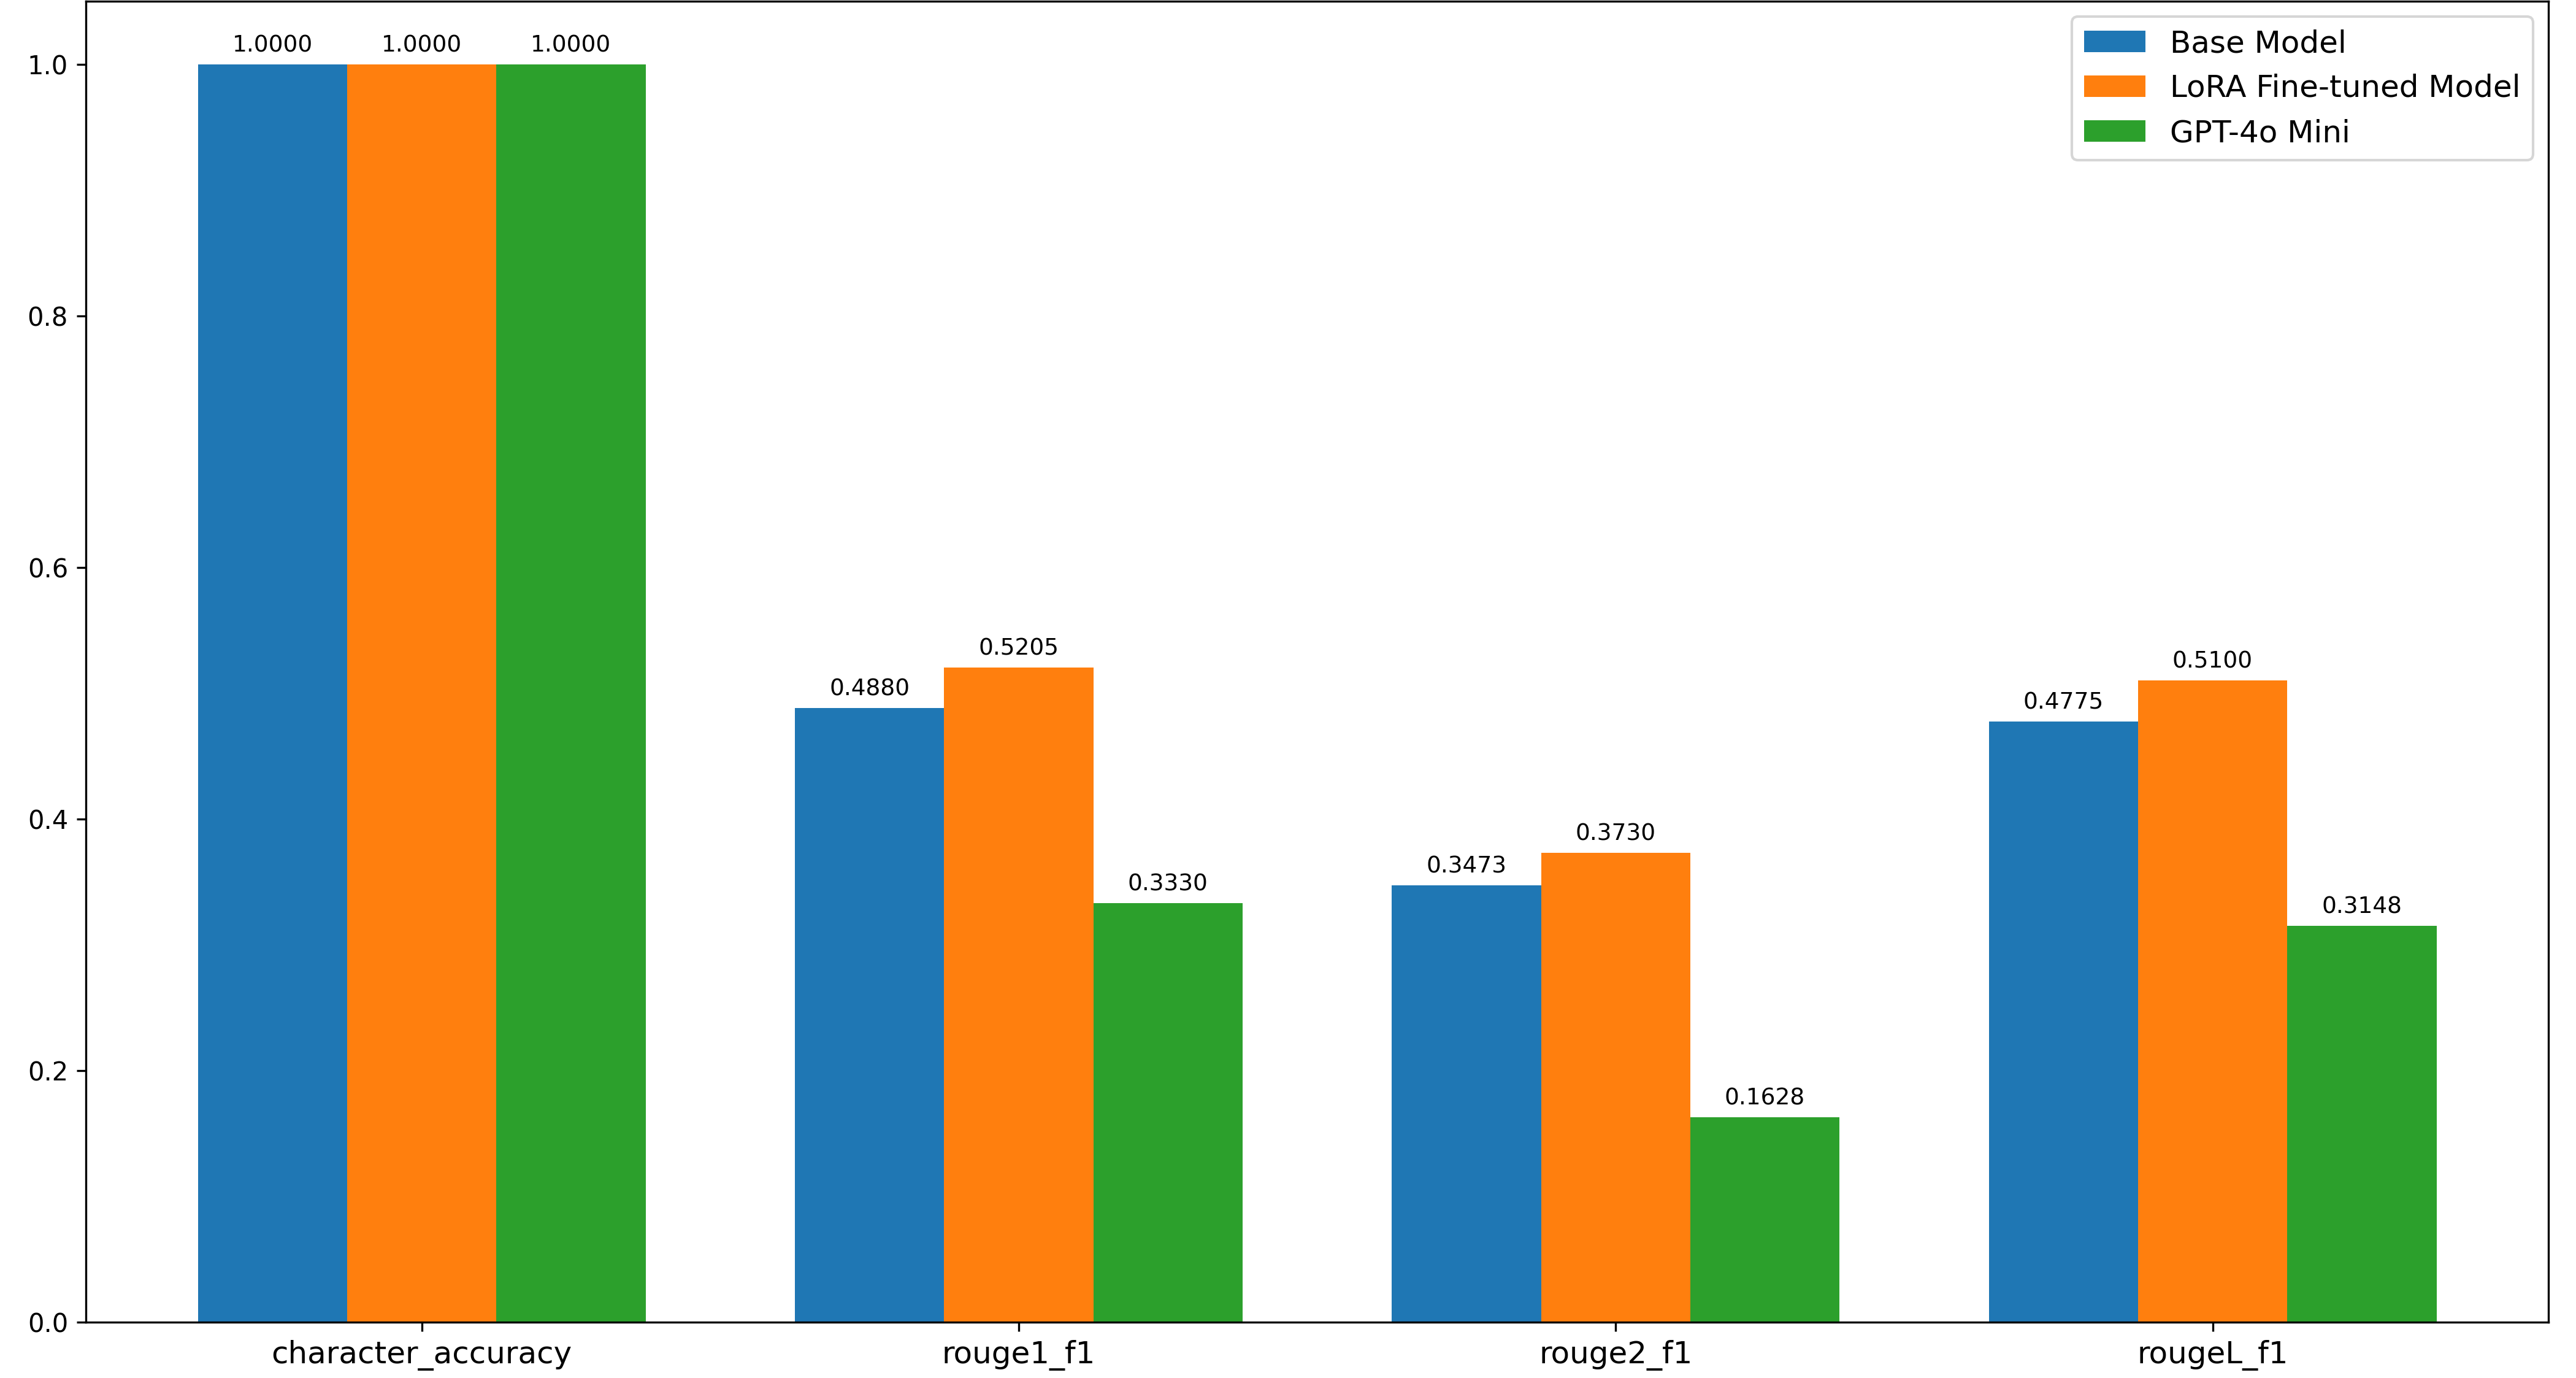
\includegraphics[width=\textwidth]{images/metrics_comparison.png}
\caption{Comparison of Metrics Across Different Models}
\label{fig:metrics_comparison}
\end{figure*}
As shown in Figure \ref{fig:metrics_comparison}, all three models achieved perfect character accuracy (1.0), indicating that they were all able to correctly identify the specific N\"{u}shu characters in the test set. This demonstrates that both the base and fine-tuned models have sufficient capability to handle the specialized character identification tasks for N\"{u}shu, which is crucial for a domain-specific knowledge system.

While character accuracy was consistent across models, significant differences emerged in the quality of the generated text. The LoRA fine-tuned model consistently outperformed both the base model and GPT-4o Mini across all ROUGE metrics, with improvements of 6.7\% in ROUGE-1 F1 (0.521 vs. 0.488), 7.4\% in ROUGE-2 F1 (0.373 vs. 0.347), and 6.8\% in ROUGE-L F1 (0.510 vs. 0.478) compared to the base model.

GPT-4o Mini showed the lowest performance across all ROUGE metrics (0.333 for ROUGE-1 F1, 0.163 for ROUGE-2 F1, and 0.315 for ROUGE-L F1), highlighting the challenges general-purpose models face with specialized domains like N\"{u}shu without proper context and fine-tuning.

These results demonstrate the effectiveness of our LoRA fine-tuning approach for the N\"{u}shu domain. The fine-tuned model's superior performance in generating accurate, relevant, and well-structured responses validates our approach of combining knowledge graph construction with targeted model adaptation. The significant performance gap between our models and GPT-4o Mini underscores the importance of domain-specific adaptation for specialized language tasks, even when compared to commercial models.


\section{Conclusion}
\label{sec:conc}
    My system integrates: (1) a Neo4j-based knowledge graph capturing N\"{u}shu character relationships; (2) a retrieval-augmented generation framework combining structured knowledge with DeepSeek-R1-Distill models; and (3) efficient domain-specific adaptation using LoRA with minimal computational overhead.

    Experimental results demonstrated the efficacy of our approach, with the LoRA-tuned model outperforming both the base model and GPT-4o Mini across all metrics (improvements of 6.7\%, 7.4\%, and 6.8\% in ROUGE-1, ROUGE-2, and ROUGE-L F1 scores respectively). While all models achieved perfect character accuracy, significant differences in text quality metrics validate the importance of domain-specific adaptation for specialized writing systems like N\"{u}shu, even when using parameter-efficient methods like LoRA.    This work contributes to digital humanities by applying modern NLP techniques to preserve endangered writing systems of cultural and historical value. Future directions include extending the knowledge graph with temporal relationships, incorporating multi-modal capabilities for processing physical manuscripts, developing cross-lingual translation beyond Chinese, and creating interactive educational tools to promote awareness of this unique cultural heritage.

    By making our system publicly available, we contribute to ongoing efforts to preserve N\"{u}shu, ensuring this remarkable writing system remains accessible to future generations. Moreover, the study of N\"{u}shu represents more than just linguistic preservation—it highlights the extraordinary wisdom that emerged under conditions of cultural deprivation, systematic gender oppression, and limited educational opportunity. 
    These insights from N\"{u}shu offer valuable lessons for contemporary society's development of equality and diversity, while demonstrating the potential of combining structured knowledge representation with neural language models for specialized domains.











\vfill\pagebreak

% References should be produced using the bibtex program from suitable
% BiBTeX files (here: strings, refs, manuals). The IEEEbib.bst bibliography
% style file from IEEE produces unsorted bibliography list.
% -------------------------------------------------------------------------
\bibliographystyle{IEEEbib}
\bibliography{refs}

\end{document}
